This study is motivated by a heat transfer driven electronic drug delivery system (EDDS) medical device, which uses applied power to heat fluid flowing through the device and into a user's mouth cavity. While the full system includes complex components such as coils for heating and an expanding mouthpiece, verifying the entire system limits the level of rigor achievable in code and solution verification due to geometric and multiphysics complexity. 

To enable systematic verification, a simplified geometry is adopted that preserves the dominant transport mechanisms of laminar flow and conjugate heat transfer while minimizing geometric complexity. This reduction enables direct comparison to analytical solutions and supports high-resolution studies. By verifying key physical processes in isolation, this approach establishes confidence in the numerical modeling framework and provides a foundation for progressively reintroducing complexity in future validation and application studies.

\subsection{Verification Framework}
Verification is divided into two categories: \textit{code verification}, which assesses the correctness of the numerical implementation through comparison with analytical solutions, and \textit{solution verification}, which quantifies numerical uncertainty arising from spatial and temporal discretizations, solver settings, and modeling assumptions. These activities follow the framework outlined in ASME V\&V 20 and V\&V 40 \cite{vv20,vv40}, and support a structured credibility assessment of simulation results for subsequent validation and decision-making.

To isolate sources of numerical error, each verification component is further subdivided according to the underlying physical processes and modeling complexity. Code verification is performed using three cases: hydrodynamic flow, radial heat conduction, and transient thermal diffusion, which independently assess the solver’s ability to reproduce fluid transport, steady thermal transport, and transient heat transfer across the fluid-solid interface. 

Solution verification is conducted using coupled fluid and thermal configurations which increase in complexity. These include a steady-state coupled pipe model and a transient, device-representative EDDS configuration. The latter provides the closest approximation to the target medical device and enables evaluation of numerical uncertainty under application relevant conditions.

\subsection{System Description \& Operating Conditions}
The pipe system is designed to approximate the geometry of the medical device, including both the internal fluid channel and surrounding casing. The fluid domain is partitioned into three regions: the pipe inlet, the pipe case, and the pipe outlet. The central pipe section, shown in Figure~\ref{fig:geometry-schematic-gen}, is thermally coupled to a surrounding solid domain representing the casing, within which volumetric heat generation is applied.

\begin{figure}[ht]
    \centering
    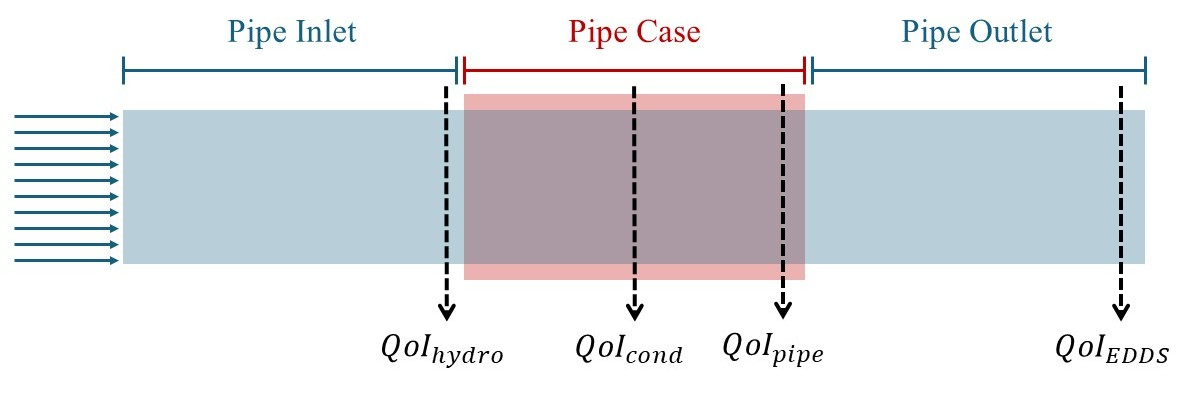
\includegraphics[width=\linewidth]{figures/schematic/schematics_verifedds_v2.jpg}
    \caption{Schematic of the generalized pipe configuration used across all verification studies.}
    \label{fig:geometry-schematic-gen}
\end{figure}

The pipe has an internal diameter of 4.54~mm and is surrounded by a casing with a thickness of 0.30~mm. Operating conditions impose a total heating power of 1~W, applied uniformly as a volumetric heat source within the casing for a duration of 10~seconds. The fluid enters with a uniform velocity of 0.5~m/s and an inlet temperature of 26.85$^\circ$C (300~K), resulting in a laminar, transient conjugate heat transfer problem involving coupled solid-fluid thermal interactions.

All verification studies introduce controlled variations in geometry, temporal regime, and quantities of interest, as summarized in Table~\ref{tab:geometry_qty}. For code verification, the configuration is intentionally simplified to isolate numerical behavior and enable comparison with analytical solutions. A sufficiently long pipe is employed to ensure fully developed hydrodynamic and thermal conditions, thereby minimizing inlet and outlet effects. 

% \begin{table*}[htbp]
%     \centering
%       \caption{Geometry quantities, in mm, for the code and solution verification studies. The pipe diameter is 4.54 mm and the case thickness is 0.30 mm.}
%     \begin{tabular}{llll|ccccc}\toprule
%               Model& Verification Study
%  &Regime&Geometry&pipe inlet&pipe case&pipe outlet& pipe &  case \\\midrule
%               Hydrodynamic& Code
%  &Steady&long pipe&45&45&0&90& 
%      45\\
%   Radial Conduction & Code
%  &Steady&medium pipe&11.375& 45& 0& 56.25& 45\\
%   Thermal Diffusion & Code
%  &Transient&medium pipe&11.375& 45& 0& 56.25& 45\\
%   Coupled Pipe& Solution
%  &Steady &long pipe&45& 45& 0& 90& 45\\
%   Simplified EDDS& Solution &Transient&short pipe&2.021& 7.2& 42.509& 51.73& 7.2\\ \bottomrule\end{tabular}
  
%     \label{tab:geometry_qty}
% \end{table*}

\begin{table*}[htbp]
    \centering
    \caption{Geometric quantities for the code and solution verification studies. All dimensions are reported in mm. The pipe diameter is 4.54 mm, and the case thickness is 0.3 mm. \(L_{\mathrm{in}}\), \(L_{\mathrm{case}}\), and \(L_{\mathrm{out}}\) denote the pipe inlet, pipe case, and pipe outlet lengths, respectively, and \(L\) denotes the total pipe length.}
    \begin{tabular}{p{2.4cm}p{1.25cm}p{1.2cm}p{1.5cm}p{3.5cm}p{3.6cm}}
        \toprule
        Study & Verification & Regime & Geometry & Physical configuration & QoI \\
        \midrule        
        Hydrodynamic
        & Code
        & Steady
        & $L_{\mathrm{in}}=45$
          $L_{\mathrm{case}}=45$ 
          $L_{\mathrm{out}}=0$
          $L=90$ 
        & Fluid only; 
          $U=0.5$ m/s;
          $p=101.325$ kPa;
        & 
          $QoI_{\mathrm{hydro}}$: Axial velocity \\
        
        \midrule
        Radial conduction
        & Code
        & Steady
        & $L_{\mathrm{in}}=11.375$
          $L_{\mathrm{case}}=56.375$ 
          $L_{\mathrm{out}}=0$
          $L=56.25$
        & Solid conduction only; Uniform heat source $S_E=3.5\times10^{8}$~W/m$^3$ &  
          $QoI_{\mathrm{cond}}$: Radial temperature solid \\
        
        \midrule
        Thermal diffusion
        & Code
        & Transient
        & $L_{\mathrm{in}}=11.375$
          $L_{\mathrm{case}}=56.375$
          $L_{\mathrm{out}}=0$
          $L=56.25$
        & Transient thermal diffusion;
          Fluid $T_0=20^\circ$C;
          Solid $T_0=30^\circ$C;
        & 
          $QoI_{\mathrm{diff}}$: Radial temperature fluid \\
        
        \midrule
        Coupled pipe
        & Solution
        & Steady
        & $L_{\mathrm{in}}=45$
          $L_{\mathrm{case}}=45$
          $L_{\mathrm{out}}=0$
          $L=90$
        & Steady conjugate heat transfer;
          $U_{\mathrm{in}}=0.5$ m/s;
          $p_{\mathrm{out}}=101.325$ kPa;
          $T_{\text{solid}}=50^\circ$C.
        & 
          $QoI_{\mathrm{pipe}}$: Bulk fluid temperature \\
        
        \midrule
        Simplified EDDS
        & Solution
        & Transient
        & $L_{\mathrm{in}}=2.021$
          $L_{\mathrm{case}}=7.2$
          $L_{\mathrm{out}}=42.509$
          $L=51.730$
        & Transient conjugate heat transfer;
          $U_{\mathrm{in}}=0.5$ m/s;
          $T_{\mathrm{in}}=26.85^\circ$C (300~K);
          $p_{\mathrm{out}}=101.325$ kPa;
          volumetric heat source applied to casing.
        &  $QoI_{\mathrm{EDDS}}$: Cross-sectional average temperature \\
        
        \bottomrule
    \end{tabular}
    \label{tab:geometry_qty}
\end{table*}


To achieve this, the pipe length is selected to exceed both the hydrodynamic and thermal entry lengths, given by

% \begin{equation}
% \small
% L_{\text{hydro}} = 0.05\,Re\,D \approx 35~\text{mm}, \quad
% L_{\text{therm}} = 0.05\,Re\,Pr\,D \approx 25~\text{mm}
% \end{equation}
\begin{equation}
\begin{aligned}
L_{\mathrm{hydro}} &= 0.05\,Re\,D \approx 35~\mathrm{mm}, \\
L_{\mathrm{therm}} &= 0.05\,Re\,Pr\,D \approx 25~\mathrm{mm},
\end{aligned}
\end{equation}
where $Re$ is the Reynolds number, $Pr$ is the Prandtl number, and $D$ is the pipe diameter. These conditions ensure fully developed flow and thermal fields and support rigorous assessment of discretization accuracy under steady-state assumptions.

In contrast, the solution verification cases are designed to more closely represent the medical device configuration. These cases incorporate increased geometric complexity and are modeled under transient conditions to capture time-dependent system behavior and assess numerical uncertainty under application relevant conditions.

\subsection{Governing Equations \& Numerical Approach}

Simulations were performed using the open-source finite-volume solver OpenFOAM. Conjugate heat transfer between the solid casing and fluid domain is modeled using the \texttt{chtMultiRegionFoam} solver, which solves the compressible Navier-Stokes equations in the fluid region, here with a constant-density equation of state, and transient heat conduction in both fluid and solid domains without phase change. Conjugate coupling is enforced at the fluid-solid interface through continuity of temperature and heat flux. All equations are discretized using the finite-volume method on unstructured hexahedral meshes.

\subsubsection*{Fluid Region}

The fluid (air) is modeled as a Newtonian fluid with constant properties under laminar flow conditions. Its density is held constant through the constant-density (\texttt{rhoConst}) equation of state, so the compressible formulation of Eqs.~\ref{eqn:conservationMass}--\ref{eqn:thermalEnergy} reduces to constant-density flow. The governing equations include conservation of mass (Eq.~\ref{eqn:conservationMass}), conservation of momentum (Eq.~\ref{eqn:conservationMomentum}), and thermal energy transport (Eq.~\ref{eqn:thermalEnergy}).

\begin{equation}\label{eqn:conservationMass}
  \dfrac{\partial \rho}{\partial t} + \nabla \cdot (\rho \mathbf{U}) = 0,
\end{equation}
\begin{equation}\label{eqn:conservationMomentum}
    \frac{\partial (\rho \mathbf{U})}{\partial t} + \nabla \cdot(\rho \mathbf{U} \mathbf{U}) = -\nabla p + \nabla \cdot \tau +\rho \mathbf{g},
\end{equation}
\begin{equation}\label{eqn:thermalEnergy}
   \frac{\partial(\rho c_p T)}{\partial t} + \nabla \cdot (\rho c_p \mathbf{U} T) = \nabla \cdot (\kappa \nabla T) + S_E,
\end{equation}
where $\mathbf{U}$ is the fluid velocity, $T$ is the temperature, $t$ is time, $\rho$ is density, $p$ is pressure, $\mathbf{g}$ is gravitational acceleration, $\tau$ is the shear stress, $c_p$ is specific heat capacity, $\kappa$ is thermal conductivity, and $S_E$ is the volumetric heat source \cite{Batchelor2000,ferziger2002cfd}.

\subsubsection*{Solid Region}
The solid casing (nickel) is modeled as an isotropic material with constant thermal properties. Transient heat conduction in the solid is governed by

\begin{equation}\label{eqn:conduction}
   \frac{\partial(\rho c_p T)}{\partial t}  = \nabla \cdot (\kappa \nabla T) + S_E.
\end{equation}
The variables $\rho$, $c_p$, $\kappa$, and $S_E$ retain the same physical interpretations as in the fluid region. At the fluid-solid interface, continuity of temperature and heat flux is enforced to ensure conjugate heat transfer.

\subsubsection*{Material Properties}
\label{subsubsec:material-properties}
Thermophysical properties used for air (fluid) and nickel (solid casing) are summarized in Table~\ref{tab:properties}; these are standard constant values for air near room temperature.

\begin{table}[htbp]
% \scriptsize
% \footnotesize
\small
\centering
\caption{Material properties used in the simulations. The air thermal conductivity follows from $\kappa = \mu c_p/Pr$ with $Pr = 0.7$, as specified in the solver input. In the steady radial conduction case, the solid density and specific heat were reduced to $\rho = 0.089$~kg/m$^3$ and $c_p = 0.00444$~J/(kg·K) to accelerate convergence to steady state; the steady solution depends only on $\kappa$.}
\label{tab:properties}
\begin{tabular}{lccc}
\toprule
\textbf{Property} & \textbf{Symbol} & \textbf{Air (fluid)} & \textbf{Nickel (solid)} \\
\midrule
Density & \( \rho \) [kg/m\textsuperscript{3}] & 1.225 & 8900 \\
Specific Heat & \( c_p \) [J/(kg·K)] & 1004.5 & 444 \\
Thermal conductivity & \( \kappa \) [W/(m·K)] & 0.0258 & 91 \\
Viscosity & \( \mu \) [Pa·s] & \( 1.8 \times 10^{-5} \) & — \\
\bottomrule
\end{tabular}
\end{table} 
% \subsubsection*{Boundary and Initial Conditions (B\&IC).}
\textit{Boundary and Initial Conditions (B\&IC).}
Boundary and initial conditions are defined to isolate the governing physical processes for each verification configuration. For code verification, simplified conditions are applied to enable comparison with analytical solutions. The hydrodynamic case assumes steady, isothermal flow with a uniform inlet velocity and fixed outlet pressure, while all walls are maintained at a constant temperature. The radial conduction case applies a uniform volumetric heat source within the solid domain with specified temperature at the outer boundary and an adiabatic interface to isolate conduction.

For solution verification, boundary conditions reflect coupled fluid-thermal behavior. The fluid enters with a uniform velocity of 0.5~m/s and a temperature of 20$^\circ$C for the coupled pipe and 26.85$^\circ$C (300~K) for the simplified EDDS, with outlet pressure fixed at 101.325~kPa and zero-gradient conditions applied to velocity and temperature. No-slip conditions are applied at all walls, and conjugate heat transfer is enforced at the fluid-solid interface. For transient simulations, both domains are initialized at the inlet temperature, with the fluid initially at rest, and a volumetric heat source is applied within the solid casing for a specified duration.

\paragraph{Numerical Discretization}
A second-order backward scheme is used for temporal discretization. Spatial discretization employs Gauss linear schemes for gradient and diffusion terms. Convective fluxes are discretized using an upwind scheme, with velocity gradients treated using Gauss upwind.

\paragraph{Solver Configuration}

The \texttt{chtMultiRegionFoam} solver employs a segregated solution strategy, in which the governing equations for fluid flow and heat transfer are solved iteratively. Pressure-velocity coupling is handled using the PIMPLE algorithm \cite{chtMultiRegion,openfoamSolvers}.

\paragraph{Parallel Implementation}
All simulations are executed in parallel using domain decomposition. Mesh partitioning is performed using the hierarchical decomposition method, and results are reconstructed using \texttt{reconstructPar} \cite{openfoam_simplegeomdecomp,openfoam_multileveldecomp,openfoam_reconstruct}.

\subsection{Quantities of Interest \& Error Metrics}
Quantities of interest (QoIs) are defined to isolate error contributions associated with each verification study (see Figure~\ref{fig:geometry-schematic-gen}). To isolate hydrodynamic error, $QoI_{\text{hydro}}$ is defined at 1.25 times the hydrodynamic entry length, ensuring fully developed flow conditions. To assess thermal conduction while minimizing boundary effects, $QoI_{\text{cond}}$ is defined at the thermal entry length. To assess the transient thermal diffusion, $QoI_{\text{diff}}$ is defined 1.2 times the thermal entry length. The steady-state coupled pipe configuration is evaluated at $QoI_{\text{pipe}}$, defined as 1.2 times the thermal entry length. For the transient, device-representative case, $QoI_{\text{EDDS}}$ is defined 1~mm upstream of the outlet to capture application-relevant behavior.

For code verification with a known analytical solution, the analytical solution is evaluated at the same spatial cross sections as the numerical solution. Pointwise comparisons are performed using the normalized $L_2$ error, defined as:

\begin{equation}
L_2 = \left( \frac{\sum_i (\phi_{i,\text{num}} - \phi_{i,\text{analytic}})^2\text{V}_i}{\sum_i (\phi_{i,\text{analytic}})^2 \text{V}_i} \right)^{1/2},
\end{equation}
where $\phi_{i,\text{num}}$ and $\phi_{i,\text{analytic}}$ represent the numerical and analytical values of the QoI at the $i$th centroid and $\text{V}_i$ is the $i$th centroid volume.

For solution verification, QoIs are compared using the relative error, defined as
\begin{equation}
Err_{\text{relative}} = \frac{|\phi_{\text{num}} - \phi_{\text{StREEQ}}|}{\phi_{\text{StREEQ}}},
\end{equation}
where $\phi_{\text{StREEQ}}$ is the extrapolated QoI obtained from the StREEQ regression method.

\subsection{Verification Study Design} 

Verification studies are designed to isolate sources of numerical error and assess solver performance across increasing levels of physical and geometric complexity. The study is divided into code verification and solution verification, followed by resolution studies used to quantify discretization error and assess solver sensitivity. A summary of the spatial and temporal resolutions used across all verification studies is provided in Table~\ref{tab:resolutions}.

\begin{table*}[htbp]
    \centering
    \caption{Spatial and temporal resolution parameters used in the verification studies.}
    \begin{tabular}{p{2.75cm}p{4.25cm}p{5.75cm}p{2.0cm}}
        \toprule
        Study & $h$ [mm] & $\Delta t$ [s] & Refinement \\
        \midrule
        Hydrodynamic
            & 0.43, 0.22, 0.11, 0.088
            & --
            & Spatial \\

        Radial conduction
            & 0.140, 0.071, 0.035
            & --
            & Spatial \\

        Thermal diffusion
            & 0.130, 0.065, 0.032
            & 0.005, 0.0005, 0.00005
            & Co-refined \\

        Coupled pipe
            & 0.43, 0.22, 0.11, 0.088
            & --
            & Spatial \\

        Simplified EDDS
            & 0.37, 0.29, 0.23, 0.18, 0.14, 0.11, 0.091
            & 0.004, 0.0035, 0.0025, 0.002, 0.0016, 0.0014, 0.001
            & Co-refined \\

        Decoupled time step
            & 0.230
            & 0.006, 0.0042, 0.003, 0.0021, 0.0015, 0.0011, 0.0007, 0.0005, 0.0004,0.0003
            & Fixed mesh \\

        Decoupled mesh
            & 0.370, 0.290, 0.230, 0.180, 0.140, 0.110, 0.091
            & 0.0050
            & Fixed time step \\

        Solver tolerance
            & 0.230
            & 0.0050
            & $10^{-3}$--$10^{-8}$ \\
        \bottomrule
    \end{tabular}
    \label{tab:resolutions}
\end{table*}

\subsubsection{Code Verification Studies}
Code verification evaluates whether the numerical implementation correctly solves the governing equations by comparison with analytical solutions. These studies are conducted in simplified configurations to isolate individual physical processes.

% All code verification studies are conducted using four progressively refined meshes with representative lengths of 0.43~mm, 0.22~mm, 0.11~mm, and 0.088~mm. These meshes are used to assess spatial convergence and enable comparison of numerical results with analytical solutions across multiple resolutions.

\paragraph{Hydrodynamic (Fluid Only) Model}
This configuration isolates fully developed laminar pipe flow (Hagen-Poiseuille flow) under steady, isothermal conditions. Heat transfer is neglected, and the pipe length is set to exceed the hydrodynamic entry length to ensure fully developed flow. The fluid enters with a uniform velocity of 0.5~m/s and temperature of 20$^\circ$C, with outlet pressure fixed at 101.325~kPa. All walls enforce no-slip conditions and are maintained at constant temperature. The QoI, $QoI_{\text{hydro}}$, is the axial velocity profile at a cross section located within the fully developed region, enabling direct comparison with the analytical solution. Spatial convergence is assessed using four progressively refined meshes with representative cell sizes of 0.43~mm, 0.22~mm, 0.11~mm, and 0.088~mm.

\paragraph{Radial Conduction Model}
This configuration isolates steady-state heat conduction in the solid domain. Fluid effects are removed by imposing an adiabatic boundary at the fluid-solid interface. A uniform volumetric heat source of 71.85 Watts is applied within the casing, and the outer wall is maintained at a fixed temperature, 293.15 K. The QoI, $QoI_{\text{cond}}$, is the radial temperature profile at the midpoint of the casing, sufficiently far from boundary effects. Spatial convergence is assessed using three progressively refined meshes with representative cell sizes of 0.14~mm, 0.071~mm, and 0.035~mm.

\paragraph{Transient Thermal Diffusion Model}
This configuration isolates transient thermal diffusion in the fluid domain by applying a zero fluid velocity, eliminating advective transport effects. The governing equation reduces to a transient diffusion problem and an analytical solution is obtained through separation of variables with Bessel functions. The fluid domain is initialized at $20^{\circ}$C, while the solid domain is initialized at $30^{\circ}$C. The QoI, $QoI_{\text{diff}}$, is the transient radial temperature profile extracted at a cross section in the fluid region at 1.2 times the thermal entry length. Spatial and temporal convergence are assessed using three co-refined meshes and time-steps with representative cell sizes of 0.13~mm, 0.065~mm, and 0.032~mm and co-refined time steps of $5\times10^{-3}$~s, $5\times10^{-4}$~s, and $5\times10^{-5}$~s.

\subsubsection{Solution Verification Studies}
Solution verification assesses numerical uncertainty in coupled fluid-thermal simulations without available analytical solutions. The study uses a set of seven mesh resolutions with corresponding characteristic cell sizes, paired with decreasing time steps to assess both spatial and temporal convergence. This range of resolutions enables evaluation of discretization error under conditions representative of the coupled fluid-thermal system.

\paragraph{Steady-State Coupled Pipe}
This configuration introduces steady-state conjugate heat transfer under laminar flow. The fluid inlet velocity and outlet pressure conditions remain consistent with the hydrodynamic case. A constant temperature, $50^{\circ} $C, is imposed within the solid region to drive thermal development. The QoI, $QoI_{\text{pipe}}$, is the bulk fluid temperature at a downstream location beyond the thermally developing region. Discretization error is quantified through mesh refinement and relative error with respect to extrapolated solutions. Spatial convergence is assessed using the same set of four progressively refined meshes employed in the code verification studies, ensuring consistency with the steady-state analytical configurations.

\paragraph{Transient Simplified EDDS}
This configuration represents a device-relevant geometry under transient conjugate heat transfer. The fluid enters at 0.5~m/s and 26.85$^\circ$C (300~K), with pressure outlet conditions and no-slip walls. A volumetric heat source is applied within the solid casing for a finite duration. The QoI, $QoI_{\text{EDDS}}$, is the cross-sectional average temperature located near the outlet, representing a measurement location relevant to the medical device usage.

Discretization error is assessed using a co-refined set of seven meshes (M1--M7) paired with progressively decreasing time steps. This design covers resolutions from coarse to very fine, enabling detailed assessment across the full discretization range. The meshes are topologically identical, geometrically similar, and globally refined with a refinement factor of $r = \sqrt[3]{2} \approx 1.26$, resulting in characteristic cell sizes of 0.37~mm (M1), 0.29~mm (M2), 0.23~mm (M3), 0.18~mm (M4), 0.14~mm (M5), 0.11~mm (M6), and 0.091~mm (M7). Each mesh is paired with a corresponding time step to maintain consistent co-refinement, with time steps of 0.004~s (T1), 0.0035~s (T2), 0.0025~s (T3), 0.002~s (T4), 0.0016~s (T5), 0.0014~s (T6), and 0.001~s (T7). The coarsest mesh (M1) is paired with the largest time step (T1), and the finest mesh (M7) with the smallest time step (T7), enabling assessment of convergence under simultaneous spatial and temporal refinement.

\paragraph{Resolution Methodology}
Discretization error is assessed through systematic refinement of spatial and temporal resolution. The steady-state studies (the hydrodynamic and radial conduction code verification cases and the coupled pipe solution verification case) employ spatial refinement only, while the transient studies (the thermal diffusion code verification case and the simplified EDDS solution verification case) use a co-refined approach in which mesh resolution and time step are reduced simultaneously (Table~\ref{tab:resolutions}).

\paragraph{Solver Tolerance} 
Solver sensitivity is assessed by varying linear solver convergence tolerances over several orders of magnitude while holding spatial and temporal resolution fixed. Convergence tolerances of $10^{-3}$, $10^{-4}$, $10^{-5}$, $10^{-6}$, $10^{-7}$, and $10^{-8}$ are evaluated at M3 and time step 0.005~s. The resulting variation in QoIs is used to quantify the influence of solver convergence criteria on numerical error. 

\subsubsection{Decoupled Resolution Analysis}
An additional analysis is performed to examine the impact of independently refining spatial and temporal resolution. Two cases are considered: (1) fixed spatial resolution with varying time step, and (2) fixed time step with varying spatial resolution. This study highlights the potential for misleading conclusions when discretization parameters are varied independently, demonstrating the importance of consistent refinement strategies in assessing convergence behavior. In Case 1, the spatial resolution is fixed at mesh M3 while the time step is systematically reduced using a refinement factor of $\sqrt{2}$. Ten time steps are evaluated: 0.0060~s, 0.0042~s, 0.0030~s, 0.0021~s, 0.0015~s, 0.0011~s, 0.0007~s, 0.0005~s, 0.0004~s, and 0.0003~s. In Case 2, the time step is fixed at 0.005~s while spatial resolution is varied using the same set of seven meshes (M1-M7) defined in the solution verification studies.

\subsection{Analytical Solutions}
\label{subsec:analytical}
Analytical solutions are used in code verification to assess whether the numerical implementation correctly represents the governing equations. Three problems are considered: fully developed laminar pipe flow, steady-state radial conduction with internal heat generation, and transient radial thermal diffusion in a fluid at rest.

\subsubsection{Hagen-Poiseuille Flow}
The analytical solution for the axial velocity profile of fully developed laminar flow in a circular pipe is given by
\begin{equation}
    u(r) = \frac{\Delta P}{4 \mu L} \left( R^2 - r^2 \right),
\label{eq:poiseuille}
\end{equation}
where $u$ is the axial velocity as a function of radial position $r$, $\Delta P$ is the pressure drop along the pipe of length $L$, $\mu$ is the dynamic viscosity, and $R$ is the pipe radius \cite{hagenPoisueille, heat_transfer}. 

\subsubsection{Radial Conduction with Internal Heat Generation}
The solid casing is modeled as a cylindrical annulus with inner radius $R$ (the pipe radius) and outer radius $r_w$. The analytical solution assumes steady-state conditions, one-dimensional radial heat conduction, constant thermal conductivity $\kappa$, uniform volumetric heat generation $S_E$, negligible axial conduction, and an adiabatic inner boundary at $r = R$.

Under these assumptions, the governing equation for steady radial conduction in cylindrical coordinates is
\begin{equation}
\frac{1}{r}\frac{d}{dr}\left(r \frac{dT}{dr}\right) + \frac{S_E}{\kappa} = 0.
\end{equation}
Integrating twice and applying the boundary conditions yields the analytical temperature distribution:
\begin{equation}
T(r) = T_w 
- \frac{S_E}{4\kappa}(r^2 - r_w^2)
+ \frac{S_E R^2}{2\kappa} 
\ln\left(\frac{r}{r_w}\right),
\label{eq:solid_conduction}
\end{equation}
where $T(r)$ is the temperature as a function of radial position, $S_E$ is the uniform volumetric heat source, $\kappa$ is the thermal conductivity, $R$ is the inner radius at the solid-fluid interface, $r_w$ is the outer wall radius, and $T_w$ is the prescribed temperature at the outer wall.

\subsubsection{Transient Thermal Diffusion Model}
The transient thermal diffusion model assumes zero fluid velocity, reducing the energy equation to a radial diffusion problem in cylindrical coordinates. The resulting governing equation is

\begin{equation}
    \frac{\partial T}{\partial t}=\alpha\left(\frac{1}{r}\frac{\partial}{\partial r}\left(r\frac{\partial T}{\partial r}\right)\right),
\label{eq:transient_diffusion}
\end{equation}
where $T$ is temperature, $t$ is time, $r$ is the radial coordinate, and $\alpha$ is the thermal diffusivity. For a cylinder the solution is written in terms of the dimensionless temperature

\begin{equation}
    \theta(r,t)=\frac{T(r,t)-T_{\text{solid}}}{T_0-T_{\text{solid}}},
\label{eq:theta_definition}
\end{equation}
where $T_0$ is the initial fluid temperature and $T_{\text{solid}}$ is the solid temperature at the fluid-solid interface, $r = R$, with $T_{\text{solid}} = T_0 + 10^{\circ}$C. Applying separation of variables gives

\begin{equation}
    \theta(r,t)=\sum_{n=1}^{\infty}\frac{2}{\lambda_n J_1(\lambda_n)}\,J_0\!\left(\frac{\lambda_n r}{R}\right)\exp\left(-\lambda_n^2 \frac{\alpha t}{R^2}\right),
\label{eq:bessel_theta_solution}
\end{equation}
where $J_0$ and $J_1$ are Bessel functions of the first kind of order zero and one, respectively, $R$ is the pipe radius, and $\lambda_n$ are the positive roots of $J_0(\lambda_n)=0$ associated with the wall temperature boundary condition. The dimensional analytical temperature is then recovered as

\begin{equation}
    T(r,t)=T_{\text{solid}}+\theta(r,t)\left(T_0 - T_{\text{solid}}\right).
\label{eq:dimensional_temperature}
\end{equation}
The analytical solution was evaluated using a truncated series expansion with $n=100$ terms. Additional sensitivity studies were performed for truncated expansions ranging from $n=5$ to $n=5000$ where errors were negligible beyond approximately $n=25$. 

While the analytical benchmark problems represent simplified physical systems, they were selected to isolate key phenomena present in the full model and provide rigorous verification targets with known solutions. Agreement with these benchmarks increases confidence in the numerical implementation of the governing equations and supports subsequent application of the model to more complex configurations. Although analytical solutions are limited to simplified representations of the underlying physics, they remain valuable verification tools for building credibility.

\subsection{Extrapolation  Method}
The \texttt{StREEQ} method is used to quantify discretization error and evaluate the convergence behavior of the numerical solution \cite{streeq_theory,streeq_git}. The method estimates the observed order of convergence and extrapolates the solution to the zero-discretization limit. When numerical error is influenced by both spatial and temporal resolution, a regression-based model is used to capture their combined contributions:
\begin{equation}
QoI(h, \Delta t) = \beta_0 + \beta_1 h^{p_h} + \beta_2 \Delta t^{p_t},
\label{eq:streeq_model_p2}
\end{equation}
where $QoI(h, \Delta t)$ is the quantity of interest as a function of representative mesh size $h$ and time step $\Delta t$, $\beta_0$ is the extrapolated solution at zero discretization, $\beta_1$ and $\beta_2$ are regression coefficients, and $p_h$ and $p_t$ are the observed orders of convergence associated with spatial and temporal refinement, respectively. This formulation does not require a constant mesh refinement factor. When only a single source of discretization error is present, the model reduces to a single-parameter regression in either $h$ or $\Delta t$.

\subsection{Reproducibility and Computational Workflow}
Reproducibility is treated as a foundational component of model credibility in this study. Verification activities rely on consistent and traceable computational processes to ensure that observed numerical behavior reflects controlled changes in resolution rather than unintended variability in model setup or execution.
All simulations and post-processing steps were performed using scripted workflows and publicly available tools to enforce consistency across verification studies. Meshes were generated using \textit{Cubit}\textsuperscript{\textregistered} version 17.04 via journal scripts to ensure consistency across refinements. The resulting Fluent-format \texttt{.msh} files were converted to OpenFOAM format using the \texttt{fluentMeshToFoam} utility. Simulations were conducted using OpenFOAM version 9 for compatibility with the SOLO high-performance computing cluster at Sandia National Laboratories~\cite{soloSNL}. Jobs were submitted using the SLURM scheduler and automated via \texttt{sbatch} scripts and Dakota 6.20~\cite{dakota}, coordinating mesh decomposition (\texttt{decomposePar}), parallel execution (\texttt{mpirun}), and solution reconstruction (\texttt{reconstructPar}). Simulations were executed on multi-core CPU nodes, with runtimes ranging from under two minutes for coarse configurations to over two days for the most refined cases. Post-processing was performed using Python 3, with analysis and visualization routines implemented using NumPy, pandas, matplotlib, and PyVista. Simulation outputs were converted from VTK format to structured \texttt{.csv} files to enable consistent extraction and analysis of quantities of interest. All computational artifacts, including mesh files, solver configurations, workflow scripts, and post-processing tools, are publicly available via a GitHub repository and archived datasets to support transparency, reproducibility, and independent verification~\cite{myRepo}. The GitHub repository can be found in \url{https://github.com/plinarodriguez/edds_verification_repo}.
